Na dane składają się wyniki ankiet zebranych pośród uczestników lekcji matematyki (395 osób) i hiszpańskiego (649 osób). Część osób (392) uzupełniło ankiety w obu grupach, dlatego należy je rozpoznać na podstawie niektórych atrybutów (informacji o szkole, miejscu zamieszkania, płci, danych o rodzinie) i usunąć ze zbioru danych. W ten sposób uzyskano 622 unikatowych wyników ankiety. W danych nie ma brakujących wartości.

Dane składają się z 33 atrybutów (zestawienie w tab. \ref{tab:attributes}), z czego 2 dotyczą spożycia alkoholu, czyli klas, które mają zostać przewidziane przez algorytmy. Na rys. \ref{fig:classes} przedstawiony został rozkład klas dla obu atrybutów dotyczących spożycia alkoholu. Można zauważyć, że zbiór, zwłaszcza dla spożycia alkoholu w weekend charakteryzuje silne niezbalansowanie klas.

\begin{figure}[h]

 \centering 
 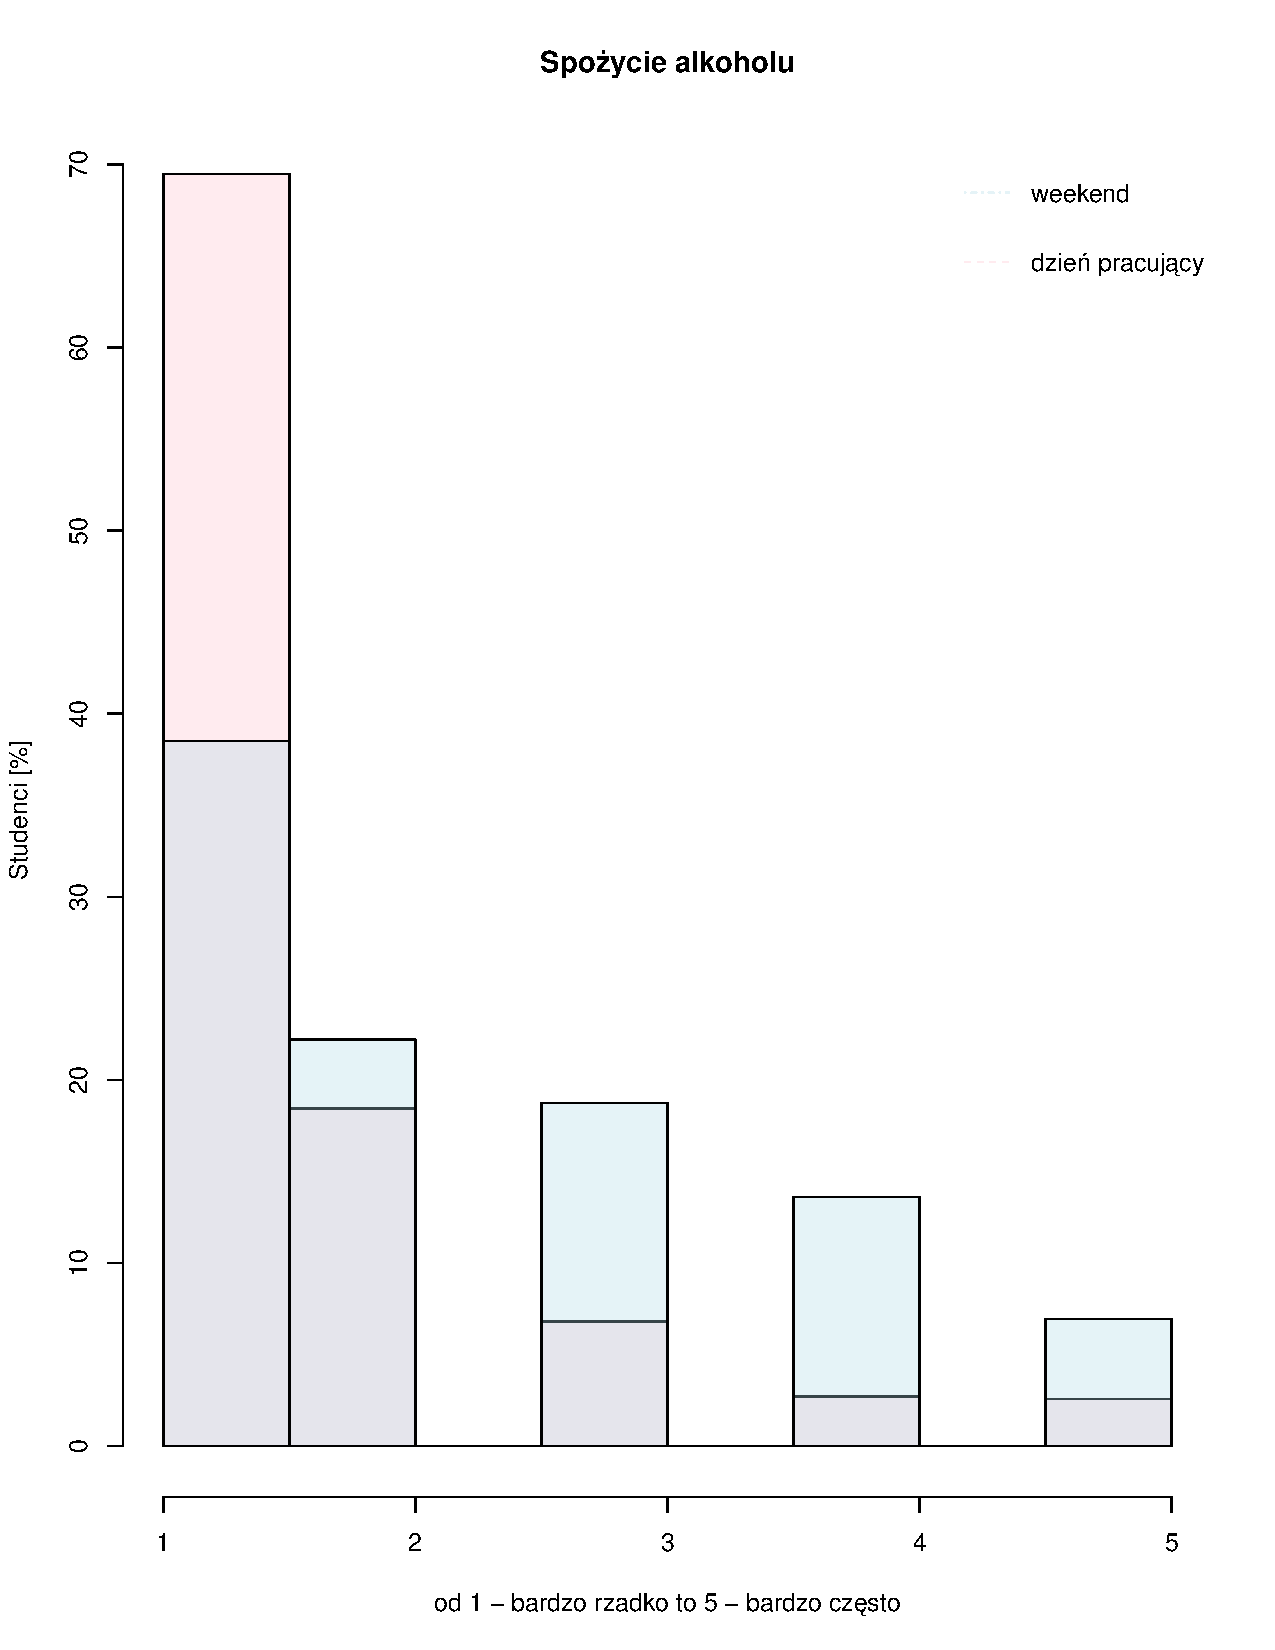
\includegraphics[scale=0.30]{tex/alc.pdf}
\caption{Rozkład klas.}
 \label{fig:classes}
\end{figure}
\begin{table}[h!]
\centering
\caption{Atrybuty analizowanych danych}
\label{tab:attributes}
\begin{tabular}{|p{1.4cm}|p{3cm}|p{3cm}|}
\hline
Nazwa & Rodzaj & Opis \\ \hline
school   &     binarny: GP lub MS &   szkoła \\ \hline
sex   &   binarny: F lub M   &   płeć \\ \hline
age   &   numeryczny (w latach)   &  wiek  \\ \hline
address   &   binarny: miasto lub wieś   &  adres zamieszkania  \\ \hline
famsize   &  binarny: większy od 3\ lub mniejszy i~równy od 3     &  ilość członków rodziny  \\ \hline
Pstatus   &  binarny: razem lub osobno    &  status zamieszkania rodziców  \\ \hline
Medu   &  numeryczny: 0-brak, 1-podstawowe,.., 5-wyższe    &   wykształcenie matki \\ \hline
Fedu   &     numeryczny: 0-brak, 1-podstawowe,.., 5-wyższe &  wykształcenie ojca  \\ \hline
Mjob   &    klasyfikacyjny: usługi, nauczyciel, lekarz, w domu, inne  &  praca matki  \\ \hline
Fjob   &    klasyfikacyjny: usługi, nauczyciel, lekarz, w domu, inne    &  praca ojca  \\ \hline
reason   &   klasyfikacyjny: reputacja, odległość od domu, kierunek(specjalność), inne   &   powód wyboru danej szkoły \\ \hline
guardian   & klasyfikacyjny: ojciec, matka, inne &  opiekun ucznia  \\ \hline
traveltime   &   numeryczny (w godzinach)    &   czas przejazdu z~domu do szkoły    \\ \hline
studytime   &   numeryczny (w godzinach)   &  czas poświęcony na naukę (tygodniowo)  \\ \hline
failures   &   numeryczny   & liczba niezdanych klas   \\ \hline
schoolsup   &  binarny: tak lub nie  & dodatkowe wsparcie edukacyjne   \\ \hline
famsup   &   binarny: tak lub nie   &   wsparcie rodziny w~nauce \\ \hline
paid  &  binarny: tak lub nie    &  dodatkowo opłacane zajęcia z danego przedmiotu  \\ \hline
activities   &  binarny: tak lub nie  &  zajęcia pozalekcyjne    \\ \hline
nursery   &   binarny: tak lub nie   &   uczęszczanie do przedszkola \\ \hline
higher   &  binarny: tak lub nie   &  plan pójścia na studia  \\ \hline
internet   &   binarny: tak lub nie   &  dostęp do Internetu w~domu  \\ \hline
romantic   &   binarny: tak lub nie   &   związek \\ \hline
famrel  &  numeryczny: 1- bardzo złe, ..., 5- bardzo dobre    & jakość relacji w~rodzinie  \\ \hline
\end{tabular}
\end{table}

\begin{figure}[h]
 \centering 
\end{figure}
\begin{table}[h!]
\begin{tabular}{|p{1.4cm}|p{3cm}|p{3cm}|}
\hline
freetime   &   numeryczny: 1- bardzo mało, ..., 5- bardzo dużo   & czas wolny po szkole   \\ \hline
gouot   &    numeryczny: 1- bardzo mało, ..., 5- bardzo dużo   &  wychodzenie z przyjaciółmi  \\ \hline
\textbf{Dalc}  &     numeryczny: 1- bardzo mało, ..., 5- bardzo dużo  & spożywanie alkoholu w tygodniu   \\ \hline
\textbf{Walc}   &    numeryczny: 1- bardzo mało, ..., 5- bardzo dużo   &  spożywanie alkoholu w weekend  \\ \hline
health   &  numeryczny: 1- bardzo zły, ..., 5- bardzo dobry    & stan zdrowia   \\ \hline
absences  &   numeryczny  &  ilość nieobecności w~szkole  \\ \hline
G1  &   numeryczny ( od 0 do 20)   &   ocena za 1.~semestr \\ \hline
G2  &   numeryczny ( od 0 do 20)     &  ocena za 2.~semestr  \\ \hline
G3   &    numeryczny ( od 0 do 20)     &  ocena końcowa  \\ \hline
\end{tabular}
\end{table}
\FloatBarrier
